% !TEX root = ../main_lecture_notes.tex
\chapter{Decentralization of blockchain system}\label{chap:decentralization}
Decentralization represents the fairness of the distribution of the accounting right of the nodes in the blockchain network. The consensus protocol must be designed so that the decision power does not eventually concentrate on a few nodes leading to a centralized system. In leader based consensus protocols, each peer is associated to a probability of being chosen. Measuring decentrality then reduces to computing the entropy of the probability distribution of the random variable equal to the peer selected  \\

\noindent \cref{sec:decentralization_pos} focuses on the \PoS protocol by modelling the evolution of the stakes of the nodes by a stochastic process with reinforcement. \cref{sec:decentralization_pow} presents the concept of mining pool and discusses the threat they represent for the decentralized aspect of the network.

\section{Decentralization in PoS}\label{sec:decentralization_pos}
The \textit{Proof-of-Stake} protocol is a leader based consensus protocol that appoints a block validator depending on how many cryptocoins he owned which corresponds to its stake. In its most basic form a coins is drawn at random, the owner of that coin appends a block and collect a reward. The stake of each peers is governed by stochastic processes with reinforcement similar to that studied in the Polya's urn problem. In Polya's urn, there are balls of various colors. At each time step a ball is drawn, the ball is then replaced in the urn together with a ball of the same color. The coins are the balls and the color is the peer that owns the balls. This analogy has been used to study the decentralization\\

\noindent Let the network be of size $p$ and denote by $r$ the reward collected at each round $n\in\mathbb{N}$ by the lucky node $x\in \{1, \ldots, p\} = E$. At time $n=0$, each peer $x\in E$ has $Z^{(x)}_0$ coins so that the total number of coins is $Z_0 = \sum_{x\in E}Z^{(x)}_0$. The number of coins owned by each peers evolve over time as
$$
Z^{(x)}_n = Z^{(x)}_0 + r\sum_{k = 1}^n\mathbb{I}_{A_{k}^{(x)}}\text{ and }Z_n = \sum_{x\in E}Z^{(x)}_n = Z_0 + nr,    
$$
where $A_{n}^{(x)}$ is the event that a coin own by peer $x\in E$ is drawn at time $n\in\mathbb{N}$. Let $(W_n^{(x)})_{n\geq0}$ be the proportion of coins owned by peer $x$ at time $n$, given by 
$$
W_n^{(x)} = \frac{Z^{(x)}_n}{Z_n}. 
$$
Let $\mathcal{F}_n = \sigma(\{Z_k^{(x)}\text{ , }x\in E, k\leq n\})$. Note that 
$$
\mathbb{P}\left(A_{n}^{(x)}|\mathcal{F}_{n-1}\right) = W_{n-1}^{(x)}.
$$
\subsection{Average stake owned by each peer}
The following result provide the average behaviour of the share of coins owned by each peer.
\begin{prop}\label{prop:average_stakes}
$$
\mathbb{E}\left(W_n^{(x)}\right) = \frac{Z_0^{(x)}}{Z_0},\text{ }x\in E\text{ }, n\geq0.
$$
\end{prop}
\begin{proof}
We show that $(W_n^{(x)})_{n\geq0}$ is a martingale. We have that 
\begin{eqnarray*}
\mathbb{E}\left[W_n^{(x)}|\mathcal{F}_{n-1}\right]&=& \mathbb{E}\left[\frac{Z^{(x)}_{n-1} + r\mathbb{I}_{A_n^{(x)}}}{Z_0 + rn}\Big \rvert\mathcal{F}_{n-1}\right]\\
&=& \frac{Z^{(x)}_{n-1} }{Z_0 + rn}+\frac{rW_{n-1}^{x}}{Z_0 + rn}\\\
&=& \frac{W_{n-1}^{(x)}[Z_0 + r(n-1)]}{Z_0 + rn}+\frac{rW_{n-1}^{x}}{Z_0 + rn}\\
&=&W_{n-1}^{x}.
\end{eqnarray*}
It then follows that 
$$
\mathbb{E}\left(W_n^{(x)}\right) = \frac{Z_0^{(x)}}{Z_0},\text{ }x\in E\text{ }, n\geq0.
$$
\end{proof}
The long term average of the stake of each peer is stable, we focus on their asymptotic distribution in the following section.
\subsection{Asymptotic distribution of the stakes}\label{ssec:stakes_distribution}
To go beyond the mean and study the distribution of the stake of the peers, we have to consider the case $r = 1$. We can then show that the joint distribution of $(W_\infty^{(1)},\ldots,  W_\infty^{(p)})$ is the Dirichlet one. 
% \begin{definition}\label{def:dirichlet}
% A random variable $X$ has a gamma distribution $\text{Gamma}(\alpha,\beta)$ if it has \pdf
% \[
% f(x) = 
% \begin{cases}
% \frac{e^{-\beta x}x^{\alpha-1}\beta^{\alpha}}{\Gamma(\alpha)},& x>0, \\
% 0,&\text{ otherwise}, 
% \end{cases}
% \]
% where $\Gamma(\alpha) = \int_0^{\infty}e^{-x}x^{\alpha-1}\text{d}x$ is the gamma function.
% \end{definition}
\begin{definition}\label{def:dirichlet}
A random vector $(W_1,\ldots, W_p)$ has a Dirichlet distribution $\text{Dir}(\alpha_1,\ldots, \alpha_p)$ if it has a joint \pdf given by 
\begin{equation}\label{eq:dirichlet_pdf}
f(w_1,\ldots, w_p;\alpha_1,\ldots, \alpha_p) = \frac{1}{B(\alpha)}\prod_{i=1}^p w_i^{\alpha_i-1}, 
\end{equation}
for $\alpha_1,\ldots, \alpha_p>0$, $0< w_1,\ldots, w_p <1$ and $\sum_{i=1}^pw_i=1$, where 
$$
B(\alpha) = \frac{\prod_{i = 1}^p \Gamma(\alpha_i)}{\Gamma(\sum_{i=1}^p \alpha_i)},
$$
and $\Gamma(\alpha) = \int_{0}^{\infty}\e^{-x}x^{\alpha-1}\text{d}x$ is the gamma function.
\end{definition}
\noindent A Dirichlet random vector can be generated by independent Gamma random variables. Recall that $X\sim\GammaDist(\alpha, \beta)$ if $X$ has \pdf
\begin{equation}\label{eq:gamma_pdf}
f_{X}(x) = \begin{cases}
\frac{e^{-\beta x}x^{\alpha-1}\beta^\alpha}{\Gamma(\alpha_i)},&
x>0\\
0,&\text{otherwise}.\end{cases}
\end{equation}

\begin{prop}\label{prop:gamma_to_dirichlet}
Let $X_i\sim \GammaDist(\alpha_i,1)$ for $i = 1,\ldots, p$ be independent random variables then 
\[
\left(\frac{X_1}{\sum_{i=1}^{p}X_i},\ldots, \frac{X_p}{\sum_{i=1}^{p}X_i}\right)\sim\text{Dir}(\alpha_1,\ldots, \alpha_p)
\]
\end{prop}
\begin{proof}
Note that because $(w_1,\ldots, w_p)$ belongs to the $p-1$ simplex then the \pdf \eqref{eq:dirichlet_pdf} may be rewritten as 
$$
f(w_1,\ldots, w_p;\alpha_1,\ldots, \alpha_p) = \frac{1}{B(\alpha)}\prod_{i=1}^{p-1} w_i^{\alpha_i-1}\left(1-\sum_{i=1}^{p-1} w_i\right)^{\alpha_p-1}, 
$$
which means that we are only interested in the distribution of the vector $\left(W_1,\ldots, W_{p-1}\right) = \left(X_{1}/\sum_{i=1}^{p}X_i,\ldots, X_{p-1}/\sum_{i=1}^{p}X_i\right)$.
Let $g:\mathbb{R}^p\mapsto \mathbb{R}^+$ be measurable and bounded and consider
\begin{eqnarray*}
&&\mathbb{E}\left[g\left(\frac{X_1}{\sum_{i=1}^{p}X_i},\ldots, \frac{X_{p-1}}{\sum_{i=1}^{p}X_i}\right)\right]\\
&=&\int_{\mathbb{R_+^p}}g\left(\frac{x_1}{\sum_{i=1}^{p}x_i},\ldots, \frac{x_{p-1}}{\sum_{i=1}^{p}x_i}\right)\frac{e^{-\sum_{i}^px_i}\prod_{i=1}^px_i^{\alpha_i-1}}{\prod_{i=1}^p\Gamma(\alpha_i)}\text{d}\lambda(x_1,\ldots, x_p)
\end{eqnarray*}
We use the change of variable 
\[
\Phi:(w_1,\ldots, w_{p-1}, v) \mapsto \left[vw_1,\ldots, vw_{p-1}, v\left(1-\sum_{i=1}^{p-1}w_i\right)\right] = \left(x_1, \ldots, x_{p-1},\sum_{i=1}^{p}x_i\right)   
\]
minding the change in the integration domain as 
$$
\Phi(\Delta_{p-1}\times \mathbb{R}_+) = \mathbb{R}^p_+ ,
$$
$\Delta_{p-1}$ is the $p-1$ simplex and the Jacobian $\left|\frac{\text{d}\Phi}{\text{d}(w_1,\ldots, w_{p-1},v)}\right|=v^{p-1}$, we get 
 \begin{eqnarray*}
 &&\mathbb{E}\left[g\left(\frac{X_1}{\sum_{i=1}^{p}X_i},\ldots, \frac{X_{p-1}}{\sum_{i=1}^{p}X_i}\right)\right]\\
&=&\int_{\Delta_{p-1}}\int_{\mathbb{R}_+}g\left(w_1,\ldots, w_{p-1}\right) \frac{e^{- v}\prod_{i=1}^{p-1}w_i^{\alpha_i-1}\left(1-\sum_{i=1}^{p-1}w_i\right)^{\alpha_p-1}v^{\sum_{i=1}^{p-1}\alpha_i-1}}
{\prod_{i=1}^p\Gamma(\alpha_i)}\text{d}\lambda(w_1,\ldots, w_{p-1}, v)\\
&=&\int_{\Delta_{p-1}}g\left(w_1,\ldots, w_{p-1}\right) \frac{\Gamma\left(\sum_{i =1}^{p}\alpha_i\right)}{\prod_{i=1}^p\Gamma(\alpha_i)}\prod_{i=1}^{p-1}w_i^{\alpha_i-1}\left(1-\sum_{i=1}^{p-1}w_i\right)^{\alpha_p-1}\text{d}\lambda(w_1,\ldots, w_{p-1}).
\end{eqnarray*} 
\end{proof}
To show that the stochastic process $(W_n^{(1)},\ldots, W_n^{(p)})$ has a Dirichlet limiting distribution we need to introduce a counting process known as Yule process.
\begin{definition}\label{def:yule_process}
A Yule process $(Y_t)_{t\geq0}$ is a pure birth process with linear birth rate given as 
\[
\mathbb{P}(Y_{t+h} = y+1|Y_{t} =y) = nh+o(h).
\] 
\end{definition}
The Yule process models the population of some particle over time, assuming that there is one particle at time $0$, so $Y_0=1$ this particle will split in two after some exponential time and this going on and on, see the illustration on \cref{fig:yule_tree}. 

%définitiondesstyles 
\tikzstyle{lien}=[-,>=stealth',rounded corners=5pt,thick] \tikzset{individu/.style={draw,thick}, individu/.default={green}} 
%définitiondel’arbre 
\begin{figure}[!ht]
\begin{center}
\begin{tikzpicture} 
\node[individu] (1) at (0,0) {}; 
\node[individu] (11) at (-3,-2) {}; 
\node[individu] (12) at (3,-2) {}; 
\node[individu] (111) at (-4.5,-4) {}; 
\node[individu] (112) at (-1.5,-4) {}; 
\node[individu] (1121) at (-2,-6.5) {}; 
\node[individu] (1122) at (-1,-6.5) {}; 
\node[individu] (121) at (1.5,-8) {}; 
\node[individu] (122) at (4.5,-8) {}; 
\draw[lien] (1) |- (-1,-1.7)  coordinate[label = {above:$\ExpDist(1)$}] -|  (11); 
\draw[lien] (1) |- (1,-1.7)-| (12); 
\draw[lien] (11) |- (-3.5,-3.7) coordinate[label = {above:$\ExpDist(1)$}]-| (111); 
\draw[lien] (11) |- (-2.5,-3.7)-| (112); 
\draw[lien] (112) |- (-1.5,-6.2) coordinate[label = {above left:$\ExpDist(1)$}]-| (1121); 
\draw[lien] (112) |- (-1.5,-6.2)-| (1122);
\draw[lien] (12) |- (2.5,-7.7) coordinate[label = {above:$\ExpDist(1)$}]-| (121); 
\draw[lien] (12) |- (3.5,-7.7)-| (122);
\draw (122) -- (4.5,-9);
\draw (121) -- (1.5,-9);
\draw (111) -- (-4.5,-9);
\draw (1121) -- (-2,-9);
\draw (1122) -- (-1,-9);
\draw[->] (-5,0) -- (-5,-10) coordinate[label = {below:$t$}] (xmax);
\draw[-, thick, dashed] (-5.5,-7) coordinate[label = {below left:$Y_t = 4$}] -- (5,-7)  (xmax);
\end{tikzpicture}
\caption{Yule tree}
\label{fig:yule_tree}
\end{center}
\end{figure}
Before moving forward, two remarks.
\begin{remark}\label{rem:yule_process_initial}
If we have $Y_0 = y_0$ particles at the initial state, then it is like starting $y_0$ independent copies of the Yule process with one particle and summing up at time $t$ the number of particles of all the Yule processes. Namely, let $(Y_t)_{t\geq0}$ be a Yule process such that $Y_0 = y_0$, then
$$
Y_t = \sum_{i = 1}^{y_0}Y_t^{(i)},
$$   
where the $Y_t^{(i)}$'s are independent Yule processes such that $Y_t^{(i)}=1$ for $i = 1,\ldots, y_0$.
\end{remark}
\begin{remark}\label{rem:stopped_yule_process}
The Yule process $(Y_t)_{t\geq0}$ is strong Markov in the sense that for any stopping time $\tau$, the stopped process 
$$
\tilde{Y}_t = Y_{\tau+t},\text{ }t\geq0
$$
is again a Yule process such that $\tilde{Y}_0 = Y_\tau$.
\end{remark}
\begin{prop}\label{prop:yule_process_dist}
Let $(Y_t)_{t\geq0}$ be a Yule process such that $Y_0 = 1$ then 
$$
\mathbb{P}(Y_t = y) = \left(1-\e^{-t}\right)^{y-1}e^{-t}.
$$

\end{prop}
\begin{proof}
The inter-arrival times $(\Delta^T_n)_{n\geq1}$ of the Yule process are independent random variable such that $\Delta^T_n = \ExpDist(n)$. If we have $n$ particles at some time $t\geq0$, that's $n$ exponential $\ExpDist(1)$ competing and a new particle appears as soon as one of them ring. We then have $\Delta^T_n = \min(X_1,\ldots, X_{n})$, where $X_1,\ldots, X_n \overset{\text{i.i.d.}}{\sim}\ExpDist(1)$ and so $\Delta^T_n \sim \ExpDist(n)$. The arrival time of the $n^{th}$ particles is given by   
$$
T_n = \sum_{k =1}^{n-1}\Delta^T_k,\text{ }n\geq2.
$$
By induction on $n\geq2$, we can show that 
\[
\mathbb{P}(T_n\leq t) = \left(1-e^{-t}\right)^{n-1}.
\]
We further deduce that 
\[
\mathbb{P}(Y_t = y) = \mathbb{P}(Y_t > y) - \mathbb{P}(Y_t > y+1) = \mathbb{P}(T_{y} \leq t) - \mathbb{P}(T_{y+1} \leq t)=\left(1-\e^{-t}\right)^{y-1}e^{-t}   
\]
\end{proof}
\begin{theo}\label{theo:convergence_yule_process}
We have that 
\[
e^{-t}Y_t\overset{\mathcal{D}}{\longrightarrow}\ExpDist(1),\text{ as }t\rightarrow \infty.
\]
\end{theo}
\begin{proof}
Let us show that $\left(e^{-t}Y_t\right)_{t\geq0}$ is a martingale. We have that, for $s\leq t$, 
\[
\mathbb{E}(e^{-t}Y_t|\mathcal{F}_s) = e^{-t}\mathbb{E}(Y_t|\mathcal{F}_s) = e^{-t}Y_se^{t-s} = e^{-s}Y_s.
\]
Because of the martingale convergence theorem, we know that $\left(e^{-t}Y_t\right)_{t\geq0}$ has a limiting distribution. Consider the Laplace transform 
\[
\mathbb{E}\left(\e^{-\theta e^{-t}Y_t}\right) = \frac{\e^{-\theta \e^{-t}}\e^{-t} }{1-\e^{-\theta \e^{-t}}(1-\e^{-t})}=\frac{1}{e^t\left(\e^{\theta\e^{-1}}-1\right)+1}\rightarrow\frac{1}{1+\theta},\text{ as }t\rightarrow\infty.
\]
which coincides with that of an exponential random variable $\ExpDist(1)$.

\end{proof}
We finally link the asymptotic behavior of the Yule processes to our initial question about the asymptotic distributions of the stakes.
\begin{theo}
We have that 
\[
\left(W_\infty^{(1)},\ldots, W_\infty^{(p)}\right)\sim\text{Dir}\left(Z_0^{(1)},\ldots, Z_0^{(p)}\right).
\]
\end{theo}
\begin{proof}
Assume that each coin owned at time $n=0$ is like the initial particle of a Yule process. That's $Z_0$ Yule processes $(Y_t^{i,j})_{t\geq0}$ for $i = 1, \ldots, Z_0^{(j)}$ and $j = 1,\ldots, p$. Each time step $n$ corresponds to the jump of one of the Yule processes $\tau_n$. The number of coins owned by peer $j=1,\ldots, p$ is then 
\[
Z_n^{(j)} = \sum_{i=1}^{Z_0^{(j)}} Y^{i,j}_{\tau_n},
\]
we have $\tau_n\rightarrow\infty$ as $n\rightarrow\infty$ and therefore 
\[
e^{-\tau_n}Z_n^{(j)} = \sum_{i=1}^{Z_0^{(j)}} Y^{i,j}_{\tau_n}e^{-\tau_n}\overset{\mathcal{D}}{\longrightarrow} \GammaDist\left(Z_0^{(j)}, 1\right),\text{ as }n\rightarrow\infty
\]
Finally 
\[
\left(W_n^{(1)},\ldots, W_n^{(p)}\right) = \left(\frac{e^{-\tau_n}Z_n^{(1)}}{\sum_{j=1}^{p}e^{-\tau_n}Z_n^{(j)}},\ldots, \frac{e^{-\tau_n}Z_n^{(p)}}{\sum_{j=1}^{p}e^{-\tau_n}Z_n^{(j)}}\right)\overset{\mathcal{D}}{\longrightarrow}\text{Dir}(Z_0^{(1)},\ldots, Z_0^{(p)})
,\text{ as }n\rightarrow\infty.
\]
\end{proof}
\begin{remark}\label{req:alternative_proof}
One can take a shorter road to show the above result. Let $(X_n)_{n\geq1}$ be the color of the ball drawn during the $n^{th}$ round. We have that 
\begin{equation}\label{eq:polya_sequence_1}
\mathbb{P}(X_1=x) = \frac{Z_0^{(x)}}{Z_{0}}
\end{equation}
and 
\begin{equation}\label{eq:polya_sequence_2}
\mathbb{P}(X_{n+1}=x) = \frac{Z_0^{(x)} + \sum_{i=1}^n\delta_{X_i}(x)}{Z_0+n} = \frac{Z_0^{(x)} + \lambda_n(x)}{Z_0+n} = m_n(x)
\end{equation}
where $\delta_{X_i}$ denotes the Dirac measure at $X_i$.
A sequence that satisfies \eqref{eq:polya_sequence_1} and \eqref{eq:polya_sequence_2} is said to be a Polya sequence with parameter $N_x\text{, }x\in E$.
\begin{lemma}
The following statements are equivalent:
\begin{itemize}
\item[(i)] $X_1,X_2,\ldots,$ is a Polya sequence
\item[(ii)] $\mu^{\ast}\sim \text{Dir}(N_x,x\in E)$ and $X_1,X_2,\ldots$ given $\mu^\ast$ are \iid as $\mu^\ast$
\end{itemize}
\end{lemma}
Consider the event $A_n = \{X_1 = x_1,\ldots, X_n = x_n\}$. Induction on $n$ allows us to show that (i) is equivalent to 
\begin{equation}\label{eq:P_A_polya_i}
\mathbb{P}(A_n) = \frac{\prod_{x\in E} \left(Z_0^{(x)}\right)^{[\lambda_n(x)]}}{Z_0^{[n]}},
\end{equation}
where $\lambda_n(x)$ is the number of $i$'s in $1,\ldots, n$ for which $x_i = x$ and $a^{[k]} = a(a+1)\ldots(a+k-1)$.  Now assume that $(ii)$ holds true, then 
$$
\mathbb{P}(A_n|\mu^\ast) = \prod_{x\in E}\mu^\ast(x)^{\lambda_n(x)},
$$
recall that $\mu^\ast$ is a random vector, indexed on $E$, We denote by $\mu^\ast(x)$ the component associated with $x\in E$. The law of total probability then yields
\begin{equation}\label{eq:P_A_polya_ii}
\mathbb{P}(A_n) = \mathbb{E}\left[\prod_{x\in E}\mu^\ast(x)^{\lambda_n(x)}\right],
\end{equation}
which is the same as \eqref{eq:P_A_polya_i}. Applying the lemma together with the law of large number yields 
$$
n^{-1}\sum_{i=1}^n\delta_{X_i}(x) \rightarrow \mu^{\ast}(x)\text{ as } n\rightarrow\infty.
$$
and then $m_n(x)\rightarrow\mu^{\ast}(x)$. This proof is taken from \citet{Blackwell1973}.
\end{remark}
The asymptotic distribution of the stakes among the peers is a Dirichlet random vector denoted by $\mu^{\ast}$ which may be considered as a probability distribution over the set of peers. Decentralization is achieved when the weights do not concentrate around a few nodes. The most desirable situation corresponds to all the peers being equally likely to be selected. It would corresponds to a uniform distribution over the set of peers which would maximizes the Shannon entropy. For $\mu^{\ast}\sim \text{Dir}(Z^{(x)}_0)$, we have 
$$
H(\mu^\ast) = -\mathbb{E}\left\{\sum_x \mu^\ast(x)\ln[\mu^\ast(x)]\right\} = -\sum_x\frac{Z_0}{Z_0^{(x)}}\left[\psi(Z_0^{(x)}+1)-\psi(Z_0+1)\right],
$$
where $\psi(x) = \frac{\text{d}}{\text{d}x}\ln[\Gamma(x)]$ is the digamma function, to be compared to $\ln(p)$.

\section{Decentralization in PoW}\label{sec:decentralization_pow}
In \cref{chap:security}, we have observed that mining blocks in a \PoW equipped blockchain is a risky business. Nodes may deviate from the prescribed protocol to counteract that but the most common way to mitigate the underlying risk is to join forces by forming mining pool. A mining pool is a joint initiative of miners that pool their computing ressources to make their capital gains more frequent and therefore have a steadier income. Consider a network of $n$ miners of hashpower $p_i, \text{ }i = 1,\ldots, n$ and assume that a subset $I\in \{1,\ldots, n\}$ decides to form a mining pool. The cumulated hashpower of this pool is then
\[
p_I = \sum_{i\in I}p_i.
\]
and the arrival rate of block rewards for a given miner $i$ rises from $p_i\cdot\lambda$ to $p_I\cdot\lambda$. Because the reward is shared among the pool participants, the size of the reward collected by miner $i$ decreases from $b$ to $p_i\cdot b$. The expected surplus is the same when mining solo and mining for a pool, but the variance (and therefore the risk) is smaller when mining for a pool. The management of a mining pool relies heavily on the reward distribution mechanism set up by a pool manager. For the redistribution system to be fair, each miner must be remunerated in proportion to her calculation effort. Miner $i$ must earn a share $p_i/p_I$
of the mining pool total income. The pool manager has to find a way to estimate the contribution of each pool participant. This is done by submitting \textit{shares} which are partial solutions to the cryptopuzzle easier to find than the actual solution. For instance, if the target is such that the hash value for finding a block must starts with $4$ leading zeros then a partial solution could be a hash value with $3$ leading zeros.  If the current difficulty of the cryptopuzzle is $D$, then the difficulty for finding a \textit{share} is set to $q\cdot D$ by the pool manager, where $q\in(0,1)$. The manager's cut is a fraction $f\in(0,1)$ of the block discovery reward $b$.\\

\noindent \cref{ssec:mining_pool_reward_system} presents the mining pool remuneration schemes and introduces the \textit{Pay-per-Share} (PpS) system on which we will focus. \cref{ssec:mining_pool_risk_analysis} defines risk models for miners and pool managers participating to a PpS pool.

\subsection{Mining pools and reward systems}\label{ssec:mining_pool_reward_system}
\subsubsection{Proportional reward system}
The proportional reward system splits time in \textit{rounds} which correspond to the time elapsed between two block discoveries. During these \textit{rounds}, the miners submit \textit{shares}. The ratio of the number of \textit{shares} submitted by miner $i$ over the total number of \textit{shares} submitted by her fellow mining pool participants determines her share of the reward and should converge to her share of the mining pool computing power, that is $p_i/p_I$ (for sufficiently low complexity of the shares, the latter limit will be a very good approximation for the actual situation indeed). The surplus of miner $i$ is then given 
\begin{equation}\label{eq:surplus_miner_proportional}
R_t^i = u - c_i\cdot t + N^I_t\cdot (1-f)\cdot \frac{p_i}{p_I}\cdot b,\text{ }t\geq0, 
\end{equation}
where $(N^I_t)$ is a Poisson proccess of intensity $p_I\cdot\lambda$ that gives the number of blocks appended to the blockchain by the mining pool. The duration of a \textit{round} is exponentially distributed $\text{Exp}\left[(p_I\lambda)^{-1}\right]$. The uncertainty on the length of the round has undesirable consequences on the time value of the \textit{shares} submitted by the miners. Indeed, if $n$ shares are submitted during a round, then the value of a given \textit{share} is $(1-f)\cdot b / n$. The longer a \textit{round} lasts, the greater the value of $n$ is. The \textit{shares} are worth less in longer rounds which triggers an exodus behavior of miners toward mining pools with shorter rounds. This phenomenon, called pool hopping, has been documented in the early work of Rosenfeld \citet{rosenfeld2011analysis}. Yet another drawback is that a miner that has found a full solution may delay the submission until her ratio of \textit{shares} submitted reflects her fraction of the mining pool computing power. The proportional system is not \textit{incentive-compatible} using the terminology of Schrijvers et al. \citet{Schrijvers2017}. A discounting factor may be applied to compensate the decreasing value of shares over time, see for instance the slush's method \citet{slush}. Now if we take a look at the risk undertaken by pool managers. Within the frame of the proportional reward system, the surplus of the pool manager is given by
\begin{equation}\label{eq:surplus_pool_manager_proportional} 
R_t^I = u + N^I_t\cdot f\cdot b,\text{ }t\geq0.
\end{equation}
Model \eqref{eq:surplus_pool_manager_proportional} does not account for any mining pool operating cost. The mining costs are entirely borne by miners and the mining pool manager only serves as coordinator. A proportional-type reward system should therefore lead to a low management fee $f$. \\

\noindent Although this system provides fairness, it has weaknesses that justify the introduction of a more sophisticated distribution mechanism. In particular, if miners seek to actually transfer some of the risk associated to the mining activity to the pool manager, then they should rather turn to a mining pool based on a \textit{Pay-per-Share} system, which is the focus of the next section.
\subsubsection{Pay-per-Share reward system}\label{eq:pps}
In a \textit{Pay-per-Share} reward system, the pool manager immediately rewards the miners for each \textit{share} submitted. Let $(M_t)_{t\geq0}$ be a Poisson process of intensity $\mu$ that counts the number of \textit{shares} submitted by the entire network of miners up to time $t\geq0$. Denote by $q\in(0,1)$ the relative difficulty of finding a block compared to finding a share. Let $0<w<b$ be the reward for finding a \textit{share}. The number of \textit{shares} submitted by miner $i$ is then a (thinned) Poisson process $(M^i_t)_{t\geq0}$ with intensity $p_i\cdot\mu$, $p_i$ being the share of the individual miner's network hashpower as defined above, and her surplus when joining a PpS mining pool becomes  
\begin{equation}\label{eq:surplus_miner_pps}
R_t^i = u - c_i\cdot t + M^i_t\cdot w,\text{ }t\geq0. 
\end{equation}
The intensities of the processes $(N_t)_{t\geq0}$ and $(M_t)_{t\geq0}$ are linked through $\lambda  = q\cdot\mu$. By setting $w=(1-f)\cdot b\cdot q$, we observe that the surplus \eqref{eq:surplus_miner_proportional} and \eqref{eq:surplus_miner_pps} have the same expectation at time $t$, but the variance and therefore the risk associated to \eqref{eq:surplus_miner_pps} is lower. This reward system has been shown to be resistant to pool hopping and is incentive compatible. It also entails a significant transfer of risk to the pool manager whose surplus process is now given by
\begin{equation}\label{eq:surplus_manager_pps}
R^I_t = u - M_t^I\cdot w + N_t^I\cdot b,\text{ }t\geq0,
\end{equation}
making her subject to the risk of bankruptcy.

\begin{remark}\label{remark_Md}
Since the process $(M_t^I)_{t\geq 0}$ requires solving for a problem of lower complexitiy than $(N_t^I)_{t\geq 0}$, ($N_t^I)_{t\geq 0}$ is a subset of the path defined by the process $(M_t^I)_{t\geq 0}$. It means that both processes are not independent. Concretely, at the moment of the block reward payment $b$, at the same time there is a realisation of the miners' reward $w$. As we sometimes need to isolate downward jumps without the simultaneous upward jump point, we define another process with a reduced intensity. We apply the superposition theorem (see e.g. \cite{Kingman1993}) to the Poisson process $M_t^I$ by redefining the down jump process as $(M_t^{I,d})_{t\geq 0} \sim Poisson(\mu_d)$, where $\mu_d = \mu-\lambda$.
\end{remark}
\noindent In addition to the bounty for finding a new block, blockchain users usually include a small financial incentive for the network to process their transaction. These transaction fees (e.g.\ referred to as \textit{gas} within the ETHEREUM blockchain), are known to be variable as they highly depend on the network congestion at a given time. Note also that since the operational cost is paid by miners using a fiat currency, it would be more accurate to account for the exchange rate of the cryptocurrency to some fiat currency. We can therefore model the successive rewards for \textit{shares} and blocks as sequences of nonnegative random variables denoted by $(W_k)_{k\geq1}$ and $(B_k)_{k\geq1}$ respectively, which for simplicity we will both assume to be \textit{i.i.d.}\  exponential variables in these notes. A reward system that features a \textit{Pay-per-Share} mechanism and includes in the miners' reward the transaction fees is referred to as a \textit{Full Pay-per-Share} reward system by practitioners. The surplus of miner $i$ in a mining pool applying the FPpS\,system is given by  
\begin{equation}\label{eq:surplus_miner_fpps}
R_t^i = u - c_i\cdot t + \sum_{k = 1}^{M^i_t}W_k,\text{ }t\geq0,
\end{equation}
and the surplus of the pool manager then becomes 
\begin{equation}\label{eq:surplus_manager_fpps}
R^I_t = u - \sum_{k = 1}^{M^I_t}W_k + \sum_{l = 1}^{N_t^I}B_l,\text{ }t\geq0. 
\end{equation}
The next section is devoted to deriving formulas for the ruin probability and expected surplus in case ruin did not occur up to a given time horizon for the models discussed above.

\subsection{Mining pool risk analysis}\label{ssec:mining_pool_risk_analysis}


\subsubsection{From the miners' viewpoint}\label{sssec:miner_viewpoint}
Consider miner $i\in \{1,\ldots, n\}$ with hashpower $p_i\in(0,1)$ that joined a FPpS mining pool $I\subset\{1,\ldots, n\}$ with relative difficulty $q\in(0,1)$ and management fee $f\in(0,1)$. Let $\lambda$ the average number of solutions published by the network per time unit and let $\mu = \lambda/q$ be the average number of partial solutions. The surplus of miner $i$ in a mining pool applying the FPpS\,system is given by
\begin{equation*}
R_t^i = u - c_i\cdot t + \sum_{k = 1}^{M^i_t}W_k,\text{ }t\geq0,
\end{equation*}
where $(M^i_t)_{t\geq0}$ is a Poisson process with intensity $\mu \cdot p_i$, and the $W_k$'s are \iid exponential variable with mean $w = (1-f)\cdot q\cdot b$. The ruin time is defined as 
$$
\tau_u^{(i)} = \inf\{t\geq0\text{ ; } R_t^i = 0\},
$$
and the net profit condition reads as 
$$
(1-f)\cdot p^{i}\cdot b\cdot \lambda>c_i.
$$
We first provide the probability distribution of $\tau_u^{i}$.
\begin{theo}\label{theo:pdf_ruin_time_miner_in_pool}
The ruin time $\tau_u^{(i)}$ takes value $t\geq u/c_i$. It has an atom of probability with 
\[
\mathbb{P}(\tau_u^{(i)} = u/c_i) = \mathbb{P}(M^{(i)}_{u/c_i}=0)=\e^{-p_i\mu u/c_i}
\]
and \pdf given by 
\begin{equation}\label{eq:pdf_ruin_time_miner_in_pool}
f_{\tau_u^{(i)}}(t)=\frac{u}{t}\mathbb{E}\left[f_{W}^{\ast M_t^{(i)}}(c_i t-u)\mathbb{I}_{M^{(i)}_t \geq1}\right]\text{, for }t\geq u/c_i.
\end{equation}
\end{theo}
\begin{proof}
Ruin is not possible before time $u/c_i$. It may occur exactly at time $t = u/c_i$ if no capital gain occur before that time. Hence we have 
$$
\mathbb{P}(\tau_u^{(i)} = u/c_i) = \mathbb{P}(M_{u/c_i} = 0) = \exp\left(-p_i\mu \frac{u}{c_i}\right).
$$
Now consider some time $t>u/c_i$. We have that 
\begin{equation*}
\{\tau_u^{(i)}\in(t,t+\text{dt})\} = \bigcup_{n = 1}^{+\infty}\left\{M_t^{(i)} = n \right\}\cap\{\tau_u^{(i)}\in(t,t+\text{dt})\},\\
\end{equation*}
and therefore
\begin{equation}\label{eq:law_of_total_prob}
\mathbb{P}\left[\tau_u^{(i)}\in(t,t+\text{dt})\right] = \sum_{n = 1}^{+\infty}\mathbb{P}\left[\tau_u^{(i)}\in(t,t+\text{dt})\big\rvert M_t^{(i)} = n\right]\mathbb{P}\left(M_t^{(i)} = n \right).
\end{equation}
Note that 
\[
\left\{M_t^{(i)} = n \right\}\cap\{\tau_u^{(i)}\in(t,t+\text{dt})\} =\left\{M_t^{(i)} = n \right\}\cap\bigcap_{k = 1}^{n}\{T_k\leq\frac{S_{k-1}+u}{c_i}\}\cap\left\{\frac{S_n+u}{c_i}\in(t,t+\text{dt})\right\}.
\]
We then have 
\begin{eqnarray*}
&&\mathbb{P}\left[\tau_u^{(i)}\in (t,t+\text{d}t)\big\rvert M_t^{(i)} = n \right]\\
&=&\mathbb{P}\left[\bigcap_{k = 1}^{n}\left\{T_k\leq\frac{S_{k-1}+u}{c_i}\right\}\cap\left\{\frac{S_n+u}{c_i}\in(t,t+\text{dt})\right\}\big\rvert M_t^{(i)} = n \right]\\
&=&\mathbb{P}\left[\bigcap_{k = 1}^{n}\left\{
U_{(k)}\leq\frac{S_{k-1}+u}{c_i t}
\right\}
\Big\rvert\frac{S_n+u}{c_i}\in(t,t+\text{dt})\right]
\mathbb{P}\left[\frac{S_n+u}{c_i}\in(t,t+\text{dt})\right]\\
&=&\mathbb{P}\left[\bigcap_{k = 1}^{n}\left\{
U_{(k)}\leq\frac{S_{k-1}+u}{c_i t}
\right\}
\Big\rvert S_{n}=c_i t -u\right]
c_i f_{W}^{\ast(n)}(c_i t -u)\\
&=&\mathbb{E}\left\{\mathbb{P}\left[\bigcap_{k = 1}^{n}\left\{
U_{(k)}\leq\frac{S_{k-1}+u}{c_i t}
\right\}\Big\rvert S_1,\ldots, S_n\right]
\Big\rvert S_{n}=c_i t -u\right\}
c_i f_{W}^{\ast(n)}(c_i t -u)\\
&=&\mathbb{E}\left\{(-1)^nG_n\left(0\Big\rvert \frac{S_0+u}{c_i t}, \ldots, \frac{S_{n-1}+u}{c_i t}\right)
\Big\rvert S_{n}=c_i t -u\right\}
c_i f_{W}^{\ast(n)}(c_i t -u)\\
&=&\frac{(-1)^n}{(c_it)^{n} }\mathbb{E}\left[G_n\left(-u\Big\rvert S_0, \ldots, S_{n-1}\right)
\Big\rvert S_{n}=c_i t -u\right]
c_i f_{W}^{\ast(n)}(c_i t -u)\\
&=&\frac{(-1)^n}{(c_it)^{n} }(-u)(-u-c_i t + u)^{n-1}
c_i f_{W}^{\ast(n)}(c_i t -u) \\
&=& \frac{u}{ t}f_{W}^{\ast(n)}(c_i t -u) .
\end{eqnarray*}
Reinserting in \eqref{eq:law_of_total_prob} yields the result.

\end{proof}
\noindent The infinite serie in \eqref{eq:pdf_ruin_time_miner_in_pool} is problematic for numerical purposes although a workable approximation may be otained by truncating it. Just like in \cref{chap:security}, we shall consider an exponential time horizon $T\sim\ExpDist(t)$ instead of a deterministic one and compute
\[
\widehat{\psi}(u,t) = \mathbb{P}(\tau_u \leq T),\text{ and }\widehat{V}(u,t) = \mathbb{E}(R_T\mathbb{I}_{\tau_u > T}).
\]
We start with the ruin probability
\begin{prop}\label{prop:rp_hat_miner_in_pool}
The ruin probability up to an exponential time horizon is given by 
\[
\widehat{\psi}(u,t) = e^{\theta^{\ast} u}
\]
where $\theta^{\ast}$ is the solution of the equation
\[
p_i\mu + 1/t - c_i \theta = p_i\mu\mathbb{E}\left(e^{-\theta W}\right)
\]
\end{prop}
\begin{proof}
Define the process
\[
S_t^{(i)} = R^{(i)}_t-u =c_i t-\sum_{k = 1}^{N_t}W_k,
\]
as it is a Levy process then the process
\[
M_t^{(i)}=\exp\left(\theta S_t^{(i)} - t\kappa(\theta)\right),
\]
is a martingale, where 
\[
\kappa(\theta) =\log \mathbb{E}(e^{\theta S_1^{(i)}}) = c_i\theta + p_i\mu \mathbb{E}\left(e^{-\theta W}\right) -\mu p_i
\]
We apply the optional stopping theorem at time $\tau_u\land T_1$, where $T_1>0$ to get 
\begin{eqnarray*}
\mathbb{E}\left(M_0^{(i)}\right) &=& \mathbb{E}\left(M_{\tau_u^{(i)}\land T_1}^{(i)}\right)\\
1 &=& \mathbb{E}\left(M_{\tau_u^{(i)}}|\tau_u^{(i)} < T_1\right)\mathbb{P}(\tau_u^{(i)} < T_1)+\mathbb{E}\left(M_T|\tau_u^{(i)} \geq T_1\right)\mathbb{P}(\tau_u^{(i)} \geq T_1)
\end{eqnarray*}
By letting $T_1\rightarrow \infty$ we get 
\begin{eqnarray*}
1 &=& \mathbb{E}\left(M_{\tau_u^{(i)}}|\tau_u^{(i)} < \infty\right)\mathbb{P}(\tau_u^{(i)} < \infty)\\
1 &=& \e^{\theta u}\mathbb{E}\left(\e^{-\kappa(\theta) \tau_u^{(i)}}|\tau_u^{(i)} < \infty\right)\mathbb{P}(\tau_u^{(i)} < \infty)
\end{eqnarray*}
Let $s>0$ and $\theta(s)$ be the unique positive solution of the equation $\kappa(\theta) =s$, then 
\begin{eqnarray*}
1 &=& \e^{\theta(s) u}\mathbb{E}\left(\e^{-\kappa(\theta(s)) \tau_u^{(i)}}|\tau_u^{(i)} < \infty\right)\mathbb{P}(\tau_u^{(i)} < \infty)\\
1 &=& \e^{\theta(s) u}\mathbb{E}\left(\e^{-s\tau_u^{(i)}}|\tau_u^{(i)} < \infty\right)\mathbb{P}(\tau_u^{(i)} < \infty)\\
1 &=& \e^{\theta(s) u}\mathbb{E}\left(\e^{-s\tau_u^{(i)}}\right)\\
\mathbb{E}\left(\e^{-s\tau_u^{(i)}}\right) &=& \e^{-\theta(s) u}\\
\end{eqnarray*}
Note that 
\[
\widehat{\psi}(u,t) = \mathbb{P}(\tau_u^{i}\geq T) = \mathbb{E}(e^{-\tau_u^{(i)}/t}) = \e^{-\theta(1/t) u}.
\]
\end{proof}
\begin{prop}\label{prop:rp_hat_miner_in_pool}
The expected wealth up to an exponential time horizon is given by 
\[
\widehat{V}(u,t) = t(c_i-p_i\mu w)e^{-\theta^{\ast} u}+u +t(p_i\mu w - c_i)
\]
where $\theta^{\ast}$ is the positive solution of the equation
\[
-c_i\theta^{2}+\theta\left(\frac{1}{t}+p_i\mu-\frac{c_i}{w}\right)+\frac{1}{wt} = 0.
\]
\end{prop}
\begin{proof}
Conditionning upon the events that may occur over th time interval $(0,h)$ with 
\begin{itemize}
    \item $T>h$ and no partial solution submitted
    \item $T\leq h$ and no partial solution submitted
    \item A partial solution submitted before $T$ and $h$
\end{itemize}
It then holds that 
\begin{eqnarray*}
\widehat{V}(u,t) &=&\e^{-h(1/t + \mu p_i)}\widehat{V}(u-ch,t)+\int_{0}^{h}\frac{1}{t}\e^{-h(1/t + \mu p_i)}(u-cs)\text{d}s\\
&+& \int_{0}^{h}\int_{0}^{+\infty}\mu p_i\e^{-h(1/t + \mu p_i)}\widehat{V}(u-cs+x,t)\frac{\e^{-x/w}}{w}\text{d}x\text{d}s.
\end{eqnarray*}
Differentiating with respect to $h$ and letting $h\rightarrow\infty$ yields
\begin{equation}\label{eq:integro_differentiql_equation_miner_in_pool}
\left(\frac{1}{t}+p_i\mu\right)\widehat{V}(u,t)+c_i\widehat{V}'(u,t)-\frac{u}{t}-\int_0^{+\infty}\widehat{V}(u+x,t)\frac{p_i\mu}{w}\e^{-x/w}\text{d}x=0,
\end{equation}
with boundary conditions \(\widehat{V}(0,t) = 0\) and \(0\leq \widehat{V}(u,t)\leq u-c_i t +p_i\mu w\). The solution is of the form 
\begin{equation}\label{eq:ansatz}
\widehat{V}(u,t) = A+Bu+C\e^{-\theta u},
\end{equation}
so that 
\begin{equation}\label{eq:ansatz_derivative}
\widehat{V}'(u,t) = B-\theta C\e^{-\theta u}.
\end{equation}
Reinserting \eqref{eq:ansatz} and \eqref{eq:ansatz_derivative} into \eqref{eq:integro_differentiql_equation_miner_in_pool}, together with the boundary condition, yields the following system of equation
\begin{equation}
\begin{cases}
\frac{A}{t}-Bp_i\mu w+Bc =0\\
B\left(\frac{1}{t}+p_i\mu\right)-\frac{1}{t}-Bp_i\mu = 0\\
\left(\frac{1}{t}+p_i\mu\right)-\theta c -\frac{p_i\mu}{1+\theta w}=0\\
A+C = 0 
\end{cases}
\end{equation}
It follows that $B = 1$, $A = t(p_i\mu w-c_i)$, $C = -A$ and $\theta^{\ast}$ is solution to 
$$
-c_i\theta^{2}+\theta\left(\frac{1}{t}+p_i\mu-\frac{c}{w}\right)+\frac{1}{wt} = 0.
$$

\end{proof}
\begin{ex}\label{ex:miner_in_pool}
Consider a miner with haspower $p = 0.01$. Let the BTC price be $\$36347.89$, and the reward be $\text{BTC}6.25 = \$248460.12$. If the time unit is the hour then $\lambda = 6$ so that one block is generated every ten minutes on average. The network consumes $10914487\text{kWh}$ per time unit. Suppose that our miner is joining a mining pool with a management fee $f = 0.05$. The ruin probability of the miner as a function of the initial reserve $u$ for a time horizon of one week is shown in \cref{fig:rp_miner_in_pool} for various relative difficulty $q = 0.25, 0.5, 0.75$.
\begin{figure}[!ht]
  \begin{center}
      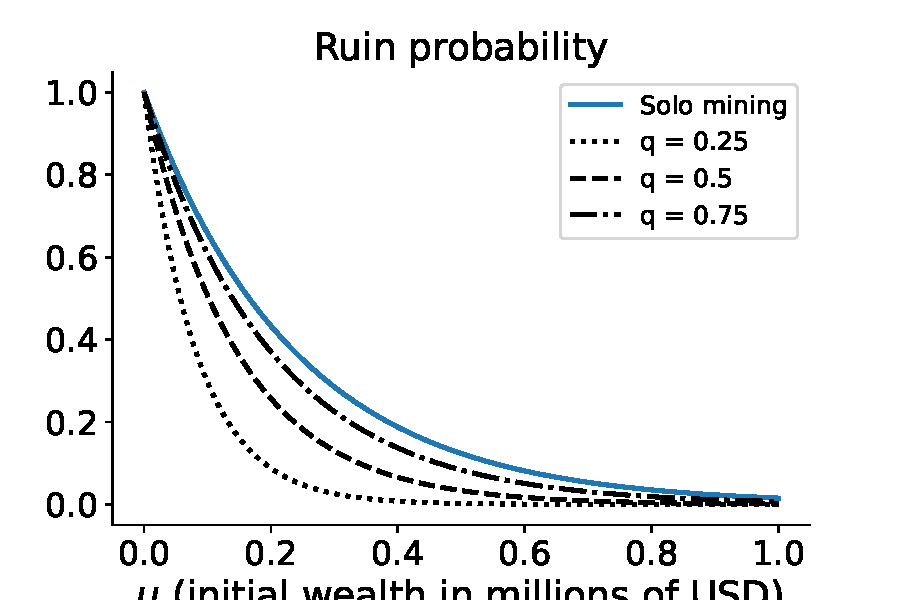
\includegraphics[width = 0.5\textwidth]{../Figures/rp_miner_in_pool}
    \caption{Ruin probability of a miner in mining pool as a function of the initial reserves depending on the relative difficulty proposed by the pool manager $q\in \{0.25, 0.5, 0.75\}$.}
    \label{fig:rp_miner_in_pool}
  \end{center}
\end{figure}
The ruin probability of a miner, mining on his own is also plotted. We see that joining a mining pool is beneficial as it reduces significantly the ruin probability.
\end{ex}


\subsubsection{From the pool manager's viewpoint}\label{ssec:manager_viewpoint}
Consider a pool manager that coordinate a FPpS mining pool $I\subset\{1,\ldots, n\}$. The manager sets the relative difficulty of finding a share compared to finding a block to $q\in(0,1)$. If we let $(N_t)_{t\geq0}$ and $(M_t)_{t\geq0}$ be Poisson processes with respective intensity $\lambda$ and $\mu$ equal to the number of block and \textit{shares} find by the network then we have $\lambda = q\mu$. Note that a \textit{share} that turns out to be a proper solution triggers a jump for both $(N_t)_{t\geq0}$ and $(M_t)_{t\geq0}$. The two processes are dependent because the paths of $(N_t)_{t\geq0}$ is a subset of the path of $(M_t)_{t\geq0}$. To isolate the jumps of the two processes we define a Poisson process $(\tilde{M}_t)_{t\geq0}$ of intensity $\mu^{\ast} = \mu -\lambda$ which corresponds to the \textit{share} that do not solve the cryptopuzzle. We have that 
\[
M_t = N_t+\tilde{M}_t,\text{ }t\geq0\text{ a.s.,}
\] 
where $N_t$ and $\tilde{M}_t$ are independent Poisson processes. The number of shares and blocks found by the pool are then thinned versions $(N_t^I)$ and $\tilde{M}_t^{I}$ of the former processes with respective intensity $p_I\lambda$ and $p_I\mu^{\ast}$. The wealth of the pool manager is given by 
\begin{equation}\label{eq:wealth_pool_manager_fpps}
R^I_t = u - \sum_{k = 1}^{\tilde{M}^I_t}\tilde{W}_k + \sum_{l = 1}^{N_t^I}\tilde{B}_l,\text{ }t\geq0, 
\end{equation}
where $\tilde{B}_l\overset{iid}{\sim}\ExpDist\left(1/b^{\ast}\right)$, $b^{\ast} = b-w$, and $W_k\overset{iid}{\sim}\ExpDist(1/w)$. The following result provides formulas for the ruin probability $\widehat{\psi}(u,t)$ and expected surplus $\widehat{V}(u,t)$ of the pool manager up to an exponential time horizon $T\sim \ExpDist(1/t)$. The ruin time is defined as 
\[
\tau_u = \inf\{t\geq0\text{ ; }R^I_t<0\},
\]
which means that the pool manager may start with no initial reserves. In the following theorem we omit the superscript $I$ and remove the $p^{I}$ from the intensities of the Poisson processes
\begin{theo}
The ruin probability is given by 
\begin{equation*}\label{psiexpe}
    \widehat{\psi}(u,t) = (1-Rw)  e^{-R u},\;u\ge 0,
\end{equation*}
and the expected profit is given by
\begin{equation*}\label{Vcombexpe}
    \widehat{V}(u,t) = (1 - Rw)[w-t(\lambda b^\ast-\mu^\ast w)] e^{-R u}+u+t(\lambda b^\ast-\mu^\ast w),
\end{equation*}
where $R$ is the (unique) solution with positive real part of 
\begin{equation*} \label{VLunde}
    -(t^{-1}+\lambda+\mu^\ast)+\lambda(1+b^\ast r)^{-1}+\mu^\ast(1-wr)^{-1}=0.
\end{equation*}
\end{theo}
\begin{proof}
Let us consider only $\widehat{V}(u,t)$ (the reasoning is the same for $\widehat{\psi}(u,t)$).
We condition upon what happen during the time interval $(0,h)$. Four possibilities
\begin{itemize}
  \item[(i)] $T>h$ and no jump during $(0,h)$
  \item[(ii)] $T<h$ and no jump over $(0,T)$
  \item[(iii)] An upward jump in the interval $(0,h)$
  \item[(iv)] A downward jump in the interval $(0,h)$
\end{itemize}
  \begin{eqnarray*}\label{neu0}
      \widehat{V}(u,t)&=& e^{-(\frac{1}{t}+\lambda+\mu^\ast)h}\widehat{V}(u,t) + \frac{1}{t}\int_0^h e^{-{s}/{t}}e^{-(\lambda +\mu^\ast) s} u\,ds\\
      & +& \lambda\int_0^he^{-\lambda s} e^{-({1}/{t}+\mu^\ast) s} \int_0^\infty\widehat{V}(u+x,t)\,dF_{B}(x)\,ds\\
      &  +&\mu^\ast \int_0^he^{-\mu^\ast s} e^{-({1}/{t}+\lambda) s}\int_0^u \widehat{V}(u-y,t) \,dF_W(y)\,ds.
  \end{eqnarray*}
  Differentiating with respect to $h$ and letting $h\rightarrow 0$ yields the following integral equation
  \begin{equation} \label{inteq}
    \lambda\int_0^\infty\widehat{V}(u+x,t)\,dF_{B}(x)-(\lambda+\mu^\ast+{1}/{t})\widehat{V}(u,t)+\mu^\ast\int_0^u \widehat{V}(u-y,t) \,dF_W(y)+{u}/{t}=0,\quad u\ge 0,
  \end{equation}
  with boundary conditions $\widehat{V}(u,t)=0$ for all $u<0$ and $0\leq\widehat{V}(u,t)\leq u+(\lambda b^\ast - \mu^\ast w)t$. Let us plug in the ansatz
  $$
  Ae^{-ru}+Bu+C
  $$
  \begin{itemize}
    \item Comparing the terms in $e^{-r u}$ gives and equation for $r$
    $$
    -(t^{-1}+\lambda+\mu^\ast)+\lambda(1+b^\ast r)^{-1}+\mu^\ast(1-wr)^{-1}=0
    $$
    of which only the positive solution $R>0$ is valid due to the boundary conditions.
    \item Comparing the terms in $u$ yields $B = 1$
    \item Comparing the terms in $1$ yields
    $$
    C = t(\lambda b^\ast-\mu^\ast w)
    $$
    \item Comparing the terms in $e^{-u/w}$
    $$
    A = (1 - Rw)[w-t(\lambda b^\ast-\mu^\ast w)]
    $$
\end{itemize}
\end{proof}

\begin{ex}\label{ex:rp_pool_manager}
Consider a mining pool with hashpower $p_I = 0.1$ and management fee $f = 0.05$. Let the BTC price be $\$36347.89$, and the reward be $\text{BTC}6.25 = \$248460.12$. If the time unit is the hour then $\lambda = 6$ so that one block is generated every ten minutes on average. \cref{fig:rp_pool_manager} displays the ruin probability of the pool manager as a function of the initial reserves depending on the relative difficulty.
\begin{figure}[!ht]
  \begin{center}
      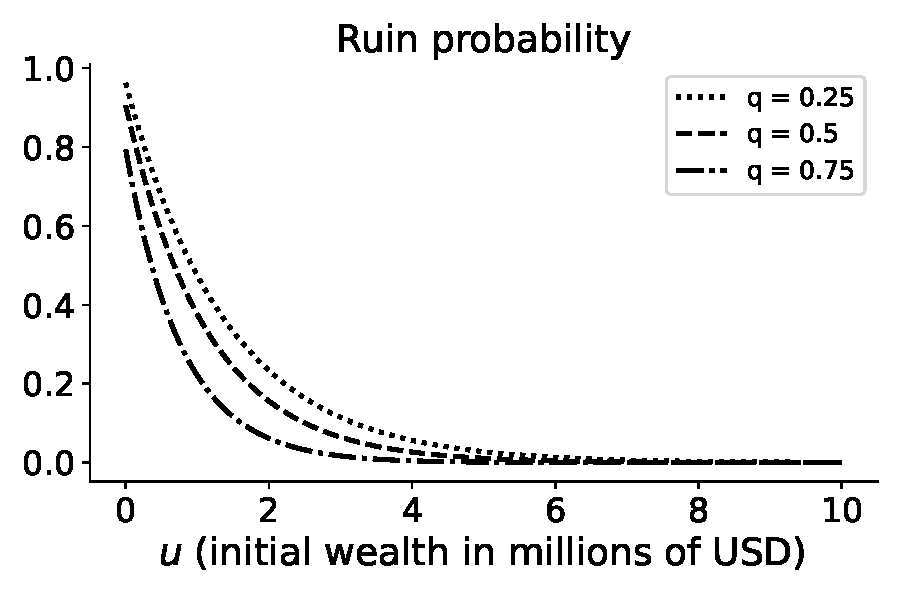
\includegraphics[width = 0.5\textwidth]{../Figures/rp_pool_manager}
    \caption{Ruin probability of a pool manager as a function of the initial reserves depending on the relative difficulty $q\in \{0.25, 0.5, 0.75\}$.}
    \label{fig:rp_pool_manager}
  \end{center}
\end{figure}
The ruin probability is higher for low relative difficulty.
\end{ex}
\subsubsection{Risk of centralization?}\label{ssec:numerical_illustrations}
Th risk of centralization exists because a mining pool that is growing larger canb reduce the management fee while maintaining the same profitability. Consider a mining pool with initial reserves $u = 10^6$ and relative difficulty $q=0.25$. The time horizon is $t = 168$ (one week). \cref{fig:level_plot_V_pool_manager_p_f} shows the expected wealth as a function of $p$ and $f$.  
\begin{figure}[!ht]
  \begin{center}
      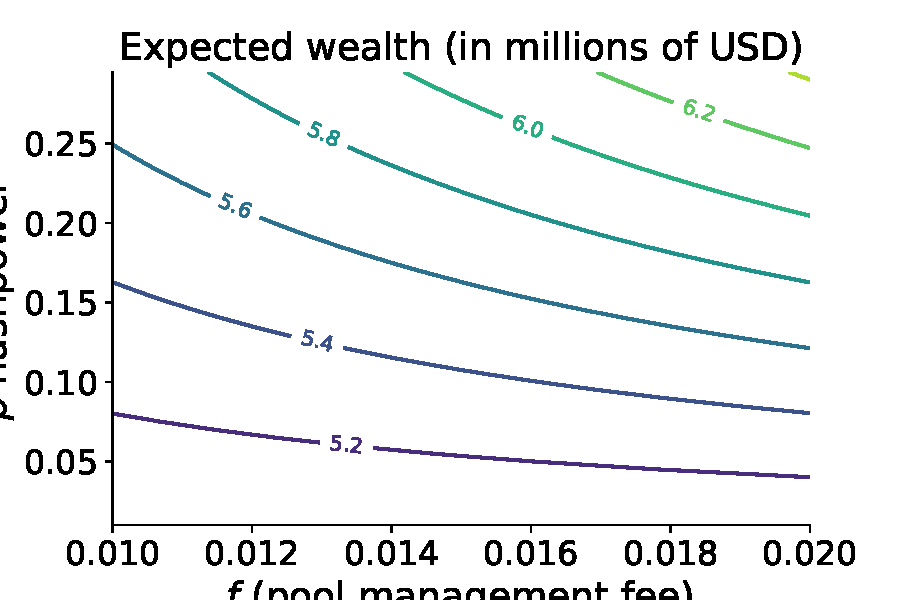
\includegraphics[width = 0.5\textwidth]{../Figures/level_plot_V_pool_manager_p_f}
    \caption{Expected wealth as a function of $p_I$ and $f$.}
    \label{fig:level_plot_V_pool_manager_p_f}
  \end{center}
\end{figure}
A large mining pool offers lower fees, thus attracts more miner and grows even larger. However a large mining pool cannot offer the same level of risk transfer than smaller mining pool. Consider two mining pool with respective hashpower $p_1 = 0.05$ and $p_2 = 0.2$ and initial reserves $u = 10^6$. The time horizon is $t = 168$ (one week). \cref{fig:level_plot_V_pool_manager_p_f} shows the expected wealth for each of these mining pool as a function of $q$ and $f$.  
\begin{figure}[!ht]
  \begin{center}
      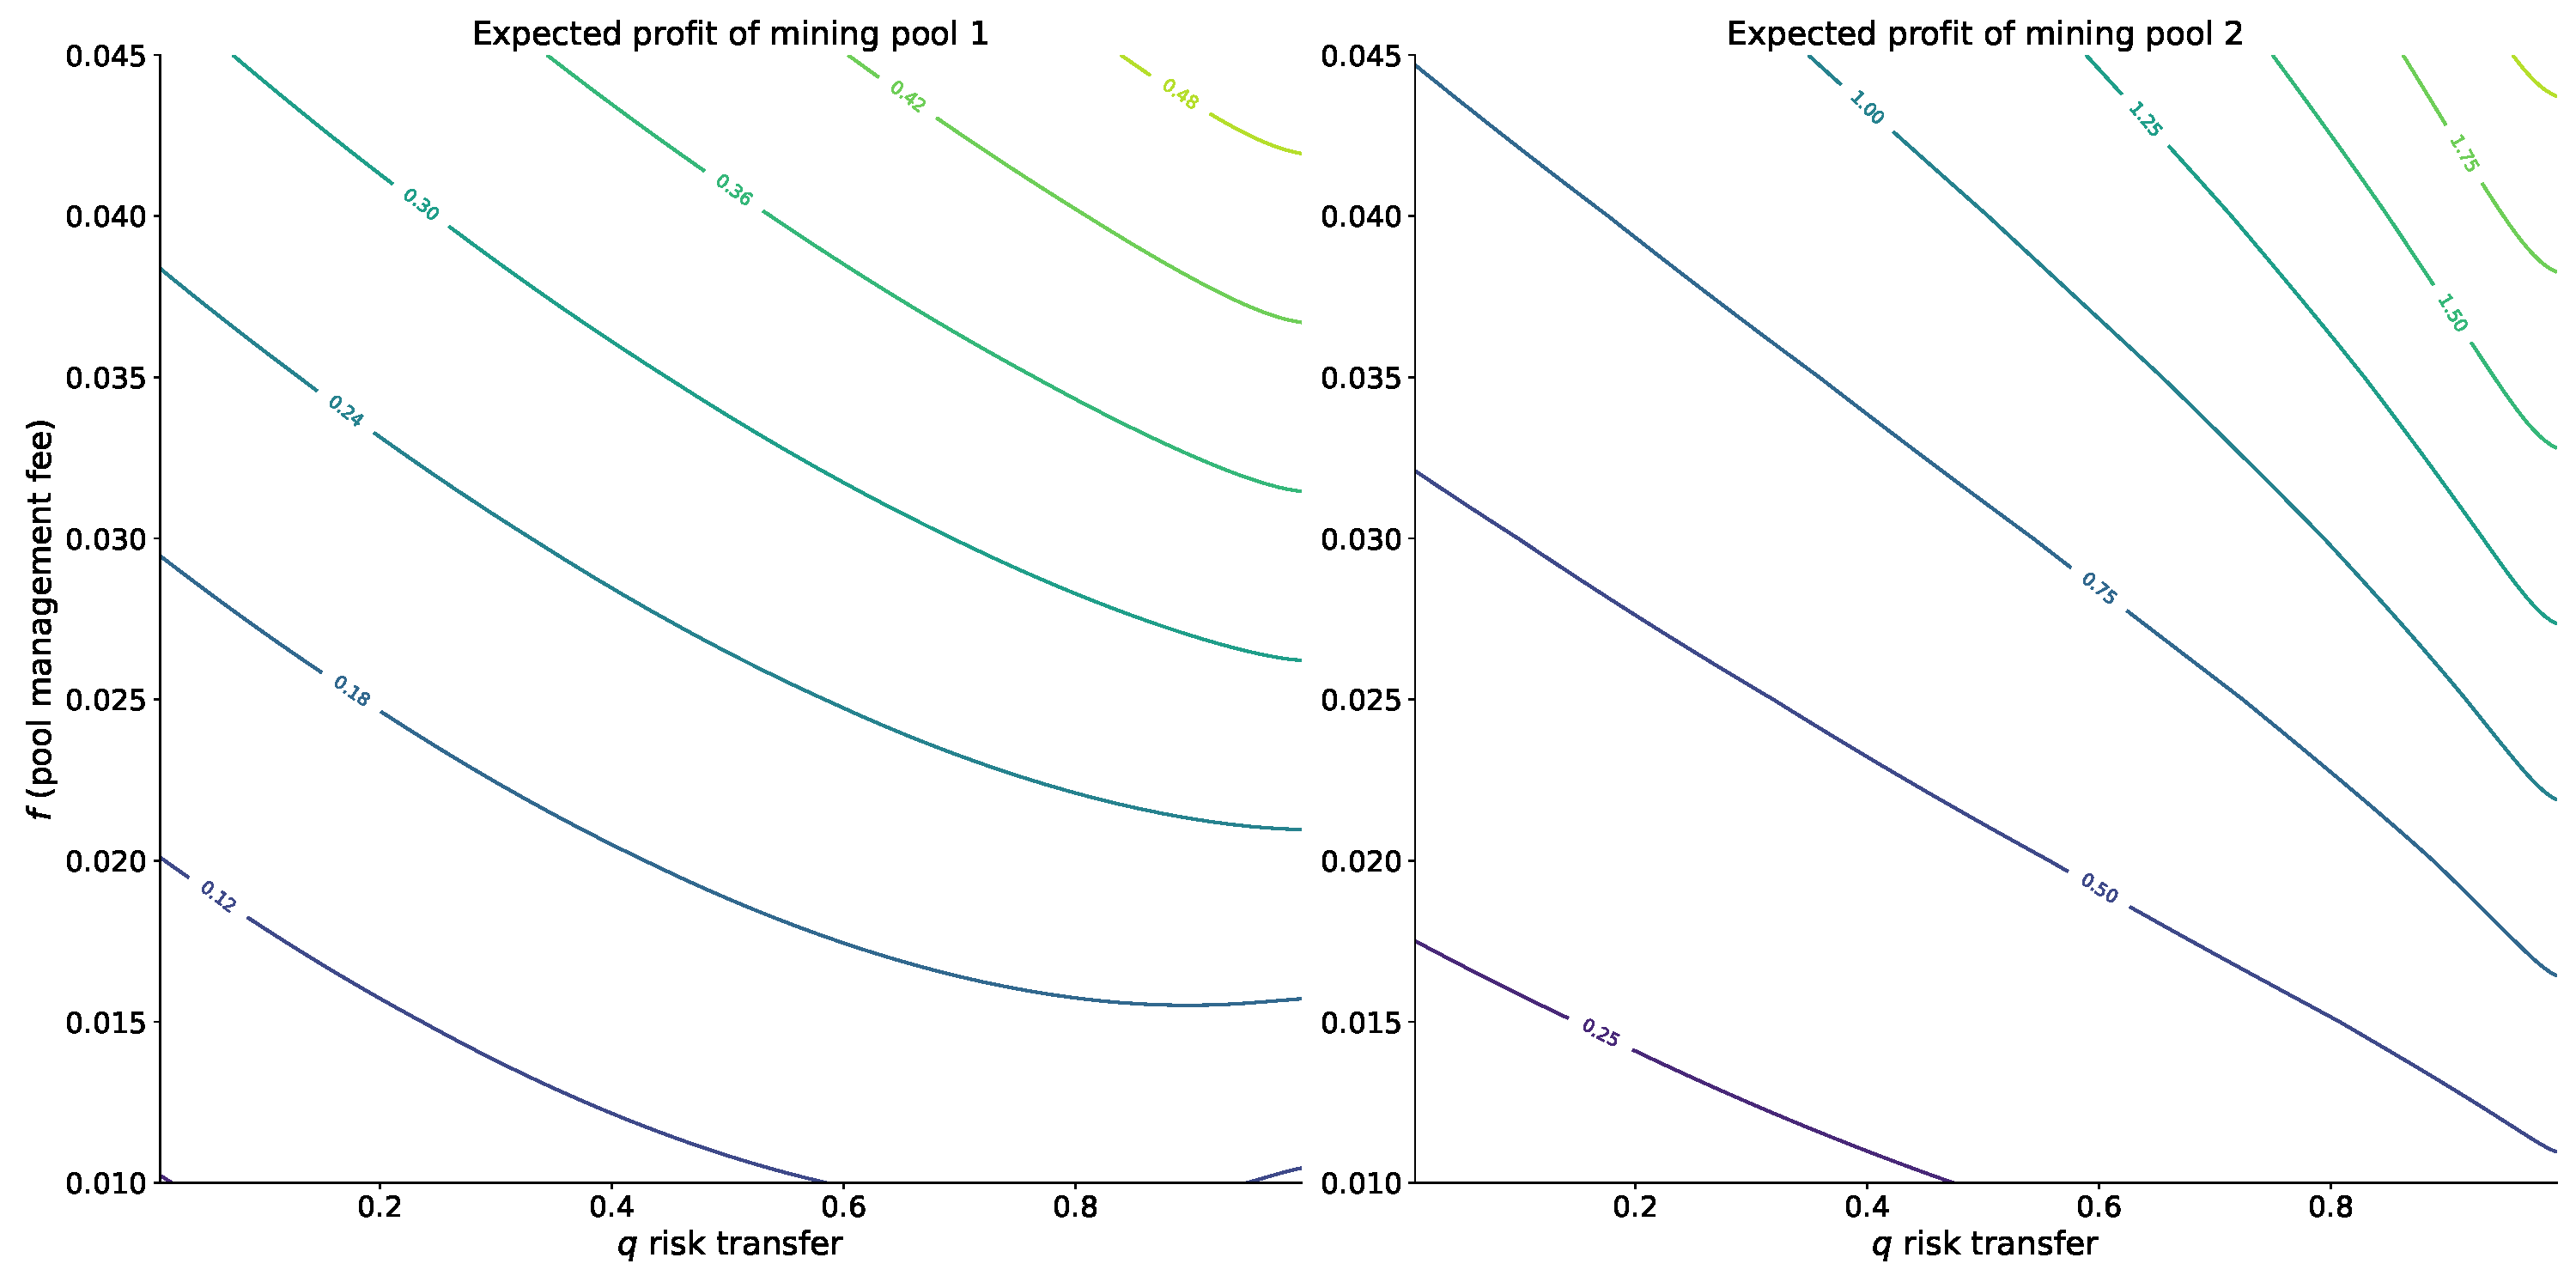
\includegraphics[width = \textwidth]{../Figures/level_plots_V_pool_manager_q_f}
    \caption{Expected wealth as a function of $p_I$ and $f$.}
    \label{fig:level_plots_V_pool_manager_q_f}
  \end{center}
\end{figure}
To offer the same level of risk transfer a larger mining pool needs to increase the fee. Centralization may prevail if the miner's preferences in terms of profitability and risk transfer are heterogenous. A game theoretic framework must be introduced to appropriately model the behaviors of the miners and mining pool manager, see the works of \citet{li2019mean} and \citet{Cong2020}.
\newpage